\documentclass[10pt,oneside]{article}
\usepackage[T1]{fontenc}
\usepackage[utf8]{inputenc}
% \usepackage{lmodern}
%\usepackage[adobe-utopia,uppercase=upright,greeklowercase=upright]{mathdesign}
\usepackage[adobe-utopia]{mathdesign}
%\usepackage{minionpro}
% \usepackage{pifont}
% \usepackage{amssymb}
\usepackage{amsmath}
\usepackage[francais]{babel}
% \usepackage[francais]{varioref}
\usepackage[dvips]{graphicx}

\usepackage{framed}
\usepackage[normalem]{ulem}
\usepackage{fancyhdr}
\usepackage{titlesec}
\usepackage{vmargin}
\usepackage{longtable}

\usepackage{ifthen}


%\usepackage{epsfig}
\usepackage{subfig}

\usepackage{multirow}
\usepackage{multicol} % Portions de texte en colonnes
\usepackage{flafter}%floatants après la référence



\usepackage{color}
\usepackage{colortbl}


\definecolor{gris25}{gray}{0.75}
\definecolor{bleu}{RGB}{18,33,98}
\definecolor{bleuf}{RGB}{42,94,171}
\definecolor{bleuc}{RGB}{231,239,247}
\definecolor{rougef}{RGB}{185,18,27}
\definecolor{rougec}{RGB}{255,230,231}
\definecolor{vertf}{RGB}{103,126,82}
\definecolor{vertc}{RGB}{220,255,191}
\definecolor{violetf}{RGB}{112,48,160}
\definecolor{violetc}{RGB}{230,224,236}

\newenvironment{sci}[1][\hsize]%
{%
    \def\FrameCommand%
    {%
%\rotatebox{90}{\textit{\textsf{Scilab}}\includegraphics[height=.8cm]{png/logo_scilab}} 
\rotatebox{90}{\includegraphics[height=.6cm]{png/logo_scilab}} 
        {\color{violetf}\vrule width 3pt}%
        \hspace{0pt}%must no space.
        \fboxsep=\FrameSep\colorbox{violetc}%
    }%
    \MakeFramed{\hsize #1 \advance\hsize-\width\FrameRestore}%
}%
{\endMakeFramed}%

\newenvironment{pseudo}[1][\hsize]%
{%
    \def\FrameCommand%
    {%
\rotatebox{90}{\textit{\textsf{Pseudo Code}}} 
        {\color{violetf}\vrule width 3pt}%
        \hspace{0pt}%must no space.
        \fboxsep=\FrameSep\colorbox{violetc}%
    }%
    \MakeFramed{\hsize #1 \advance\hsize-\width\FrameRestore}%
}%
{\endMakeFramed}%

\newenvironment{py}[1][\hsize]%
{%
    \def\FrameCommand%
    {%
%\rotatebox{90}{\textit{\textsf{Python}}} 
\rotatebox{90}{\includegraphics[height=.6cm]{png/logo_python}} 
        {\color{violetf}\vrule width 3pt}%
        \hspace{0pt}%must no space.
        \fboxsep=\FrameSep\colorbox{violetc}%
    }%
    \MakeFramed{\hsize #1 \advance\hsize-\width\FrameRestore}%
}%
{\endMakeFramed}%


\newenvironment{corrige}[1][\hsize]%
{%
    \def\FrameCommand
    {%
\rotatebox{90}{\textit{\textsf{Correction}}} 
        {\color{violetf}\vrule width 3pt}%
        \hspace{0pt}%must no space.
        \fboxsep=\FrameSep\colorbox{violetc}%
    }%
    \MakeFramed{\hsize#1\advance\hsize-\width\FrameRestore}%
}%
{\endMakeFramed}%



\newenvironment{rem}[1][\hsize]%
{%
    \def\FrameCommand
    {%
\rotatebox{90}{\textit{\textsf{Remarque}}} 
        {\color{bleuf}\vrule width 3pt}%
        \hspace{0pt}%must no space.
        \fboxsep=\FrameSep\colorbox{bleuc}%
    }%
    \MakeFramed{\hsize#1\advance\hsize-\width\FrameRestore}%
}%
{\endMakeFramed}%


\newenvironment{savoir}[1][\hsize]%
{%
    \def\FrameCommand
    {%
\rotatebox{90}{\textit{\textsf{Savoir}}} 
        {\color{bleuf}\vrule width 3pt}%
        \hspace{0pt}%must no space.
        \fboxsep=\FrameSep\colorbox{bleuc}%
    }%
    \MakeFramed{\hsize#1\advance\hsize-\width\FrameRestore}%
}%
{\endMakeFramed}%

\newenvironment{prob}[1][\hsize]%
{%
    \def\FrameCommand%
    {%
\rotatebox{90}{\textit{\textsf{ Problématique}}} 
        {\color{rougef}\vrule width 3pt}%
        \hspace{0pt}%must no space.
        \fboxsep=\FrameSep\colorbox{rougec}%
    }%
    \MakeFramed{\hsize#1\advance\hsize-\width\FrameRestore}%
}%
{\endMakeFramed}%

\newenvironment{obj}[1][\hsize]%
{%
    \def\FrameCommand%
    {%
\rotatebox{90}{\textit{\textsf{ $\;$}}} 
        {\color{rougef}\vrule width 3pt}%
        \hspace{0pt}%must no space.
        \fboxsep=\FrameSep\colorbox{rougec}%
    }%
    \MakeFramed{\hsize#1\advance\hsize-\width\FrameRestore}%
}%
{\endMakeFramed}%

\newenvironment{defi}[1][\hsize]%
{%
    \def\FrameCommand%
    {%
\rotatebox{90}{\textit{\textsf{Définition\\}}} 
        {\color{bleuf}\vrule width 3pt}%
        \hspace{0pt}%must no space.
        \fboxsep=\FrameSep\colorbox{bleuc}%
    }%
    \MakeFramed{\hsize#1\advance\hsize-\width\FrameRestore}%
}%
{\endMakeFramed}%


\newenvironment{demo}[1][\hsize]%
{%
    \def\FrameCommand%
    {%
\rotatebox{90}{\textit{\textsf{Démonstration\\}}} 
        {\color{bleuf}\vrule width 3pt}%
        \hspace{0pt}%must no space.
        \fboxsep=\FrameSep\colorbox{bleuc}%
    }%
    \MakeFramed{\hsize#1\advance\hsize-\width\FrameRestore}%
}%
{\endMakeFramed}%


\newenvironment{hypo}[1][\hsize]%
{%
    \def\FrameCommand%
    {%
\rotatebox{90}{\textit{\textsf{Hypothèse\\}}} 
        {\color{bleuf}\vrule width 3pt}%
        \hspace{0pt}%must no space.
        \fboxsep=\FrameSep\colorbox{bleuc}%
    }%
    \MakeFramed{\hsize#1\advance\hsize-\width\FrameRestore}%
}%
{\endMakeFramed}%


\newenvironment{prop}[1][\hsize]%
{%
    \def\FrameCommand%
    {%
\rotatebox{90}{\textit{\textsf{Propriété\\}}} 
        {\color{bleuf}\vrule width 3pt}%
        \hspace{0pt}%must no space.
        \fboxsep=\FrameSep\colorbox{bleuc}%
    }%
    \MakeFramed{\hsize#1\advance\hsize-\width\FrameRestore}%
}%
{\endMakeFramed}%

\newenvironment{props}[1][\hsize]%
{%
    \def\FrameCommand%
    {%
\rotatebox{90}{\textit{\textsf{Propriétés\\}}} 
        {\color{bleuf}\vrule width 3pt}%
        \hspace{0pt}%must no space.
        \fboxsep=\FrameSep\colorbox{bleuc}%
    }%
    \MakeFramed{\hsize#1\advance\hsize-\width\FrameRestore}%
}%
{\endMakeFramed}%

\newenvironment{exemple}[1][\hsize]%
{%
    \def\FrameCommand%
    {%
\rotatebox{90}{\textit{\textsf{Exemple\\}}} 
        {\color{vertf}\vrule width 3pt}%
        \hspace{0pt}%must no space.
        \fboxsep=\FrameSep\colorbox{vertc}%
    }%
    \MakeFramed{\hsize#1\advance\hsize-\width\FrameRestore}%
}%
{\endMakeFramed}%

\newenvironment{resultat}[1][\hsize]%
{%
    \def\FrameCommand%
    {%
\rotatebox{90}{\textit{\textsf{Résultat\\}}} 
        {\color{rougef}\vrule width 3pt}%
        \hspace{0pt}%must no space.
        \fboxsep=\FrameSep\colorbox{rougec}%
    }%
    \MakeFramed{\hsize#1\advance\hsize-\width\FrameRestore}%
}%
{\endMakeFramed}%

\newenvironment{methode}[1][\hsize]%
{%
    \def\FrameCommand%
    {%
\rotatebox{90}{\textit{\textsf{Méthode\\}}} 
        {\color{rougef}\vrule width 3pt}%
        \hspace{0pt}%must no space.
        \fboxsep=\FrameSep\colorbox{rougec}%
    }%
    \MakeFramed{\hsize#1\advance\hsize-\width\FrameRestore}%
}%
{\endMakeFramed}%

\newenvironment{theo}[1][\hsize]%
{%
    \def\FrameCommand%
    {%
\rotatebox{90}{\textit{\textsf{Théorème\\}}} 
        {\color{rougef}\vrule width 3pt}%
        \hspace{0pt}%must no space.
        \fboxsep=\FrameSep\colorbox{rougec}%
    }%
    \MakeFramed{\hsize#1\advance\hsize-\width\FrameRestore}%
}%
{\endMakeFramed}%

\newenvironment{warn}[1][\hsize]%
{%
    \def\FrameCommand%
    {%
\rotatebox{90}{\textit{\textsf{Attention\\}}} 
        {\color{rougef}\vrule width 3pt}%
        \hspace{0pt}%must no space.
        \fboxsep=\FrameSep\colorbox{rougec}%
    }%
    \MakeFramed{\hsize#1\advance\hsize-\width\FrameRestore}%
}%
{\endMakeFramed}%

% \usepackage{pstricks}
%\usepackage{minitoc}
% \setcounter{minitocdepth}{4}

\setcounter{tocdepth}{2}

% \mtcselectlanguage{french} 

%\usepackage{draftcopy}% "Brouillon"
% \usepackage{floatflt}
\usepackage{psfrag}
%\usepackage{listings} % Permet d'insérer du code de programmation
\renewcommand{\baselinestretch}{1.2}

% Changer la numérotation des figures :
% ------------------------------------
% \makeatletter
% \renewcommand{\thefigure}{\ifnum \c@section>\z@ \thesection.\fi
%  \@arabic\c@figure}
% \@addtoreset{figure}{section}
% \makeatother
 


%%%%%%%%%%%%
% Définition des vecteurs %
%%%%%%%%%%%%
 \newcommand{\vect}[1]{\overrightarrow{#1}}

%%%%%%%%%%%%
% Définition des torseusr %
%%%%%%%%%%%%

 \newcommand{\torseur}[1]{%
\left\{{#1}\right\}
}

\newcommand{\torseurcin}[3]{%
\left\{\mathcal{#1} \left(#2/#3 \right) \right\}
}

\newcommand{\torseurstat}[3]{%
\left\{\mathcal{#1} \left(#2\rightarrow #3 \right) \right\}
}

 \newcommand{\torseurc}[8]{%
%\left\{#1 \right\}=
\left\{
{#1}
\right\}
 = 
\left\{%
\begin{array}{cc}%
{#2} & {#5}\\%
{#3} & {#6}\\%
{#4} & {#7}\\%
\end{array}%
\right\}_{#8}%
}

 \newcommand{\torseurcol}[7]{
\left\{%
\begin{array}{cc}%
{#1} & {#4}\\%
{#2} & {#5}\\%
{#3} & {#6}\\%
\end{array}%
\right\}_{#7}%
}

 \newcommand{\torseurl}[3]{%
%\left\{\mathcal{#1}\right\}_{#2}=%
\left\{%
\begin{array}{l}%
{#1} \\%
{#2} %
\end{array}%
\right\}_{#3}%
}

 \newcommand{\vectv}[3]{%
\vect{V\left( {#1} \in {#2}/{#3}\right)}
}


\newcommand{\vectf}[2]{%
\vect{R\left( {#1} \rightarrow {#2}\right)}
}

\newcommand{\vectm}[3]{%
\vect{\mathcal{M}\left( {#1}, {#2} \rightarrow {#3}\right)}
}


 \newcommand{\vectg}[3]{%
\vect{\Gamma \left( {#1} \in {#2}/{#3}\right)}
}

 \newcommand{\vecto}[2]{%
\vect{\Omega\left( {#1}/{#2}\right)}
}
% }$$\left\{\mathcal{#1} \right\}_{#2} =%
% \left\{%
% \begin{array}{c}%
%  #3 \\%
%  #4 %
% \end{array}%
% \right\}_{#5}}

%  ------------------------------------------
% | Modification du formatage des sections : | 
%  ------------------------------------------

% Grands titres :
% ---------------

\newcommand{\titre}[1]{%
\begin{center}
      \bigskip
      \rule{\textwidth}{1pt}
      \par\vspace{0.1cm}
      
      \textbf{\large #1}
      \par\rule{\textwidth}{1pt}
    \end{center}
    \bigskip
  }

% Supprime le numéro du chapitre dans la numérotation des sections:
% -----------------------------------------------------------------
\makeatletter
\renewcommand{\thesection}{\@arabic\c@section}
\makeatother


% \titleformat{\chapter}[display]
% {\normalfont\Large\filcenter}
% {}
% {1pc}
% {\titlerule[1pt]
%   \vspace{1pc}%
%   \Huge}[\vspace{1ex}%
% \titlerule]


%%%% Chapitres Comme PY Pechard %%%%%%%%%
% numéro du chapitre
\DeclareFixedFont{\chapnumfont}{OT1}{phv}{b}{n}{80pt}
% pour le mot « Chapitre »
\DeclareFixedFont{\chapchapfont}{OT1}{phv}{m}{it}{40pt}
% pour le titre
\DeclareFixedFont{\chaptitfont}{T1}{phv}{b}{n}{25pt}

\definecolor{gris}{gray}{0.75}
\titleformat{\chapter}[display]%
	{\sffamily}%
	{\filleft\chapchapfont\color{gris}\chaptertitlename\
	\\
	\vspace{12pt}
	\chapnumfont\thechapter}%
	{16pt}%
	{\filleft\chaptitfont}%
	[\vspace{6pt}\titlerule\titlerule\titlerule]

%%%%  Fin Chapitres Comme PY Pechard %%%%%%%%%


% Section, subsection, subsubsection sans serifs :
% % ----------------------------------------------

% \makeatletter
% \renewcommand{\section}{\@startsection{section}{0}{0mm}%
% {\baselineskip}{.3\baselineskip}%
% {\normalfont\sffamily\Large\textbf}}%
% \makeatother

\makeatletter
\renewcommand{\@seccntformat}[1]{{\textcolor{bleu}{\csname
the#1\endcsname}\hspace{0.5em}}}
\makeatother

\makeatletter
\renewcommand{\section}{\@startsection{section}{1}{\z@}%
                       {-4ex \@plus -1ex \@minus -.4ex}%
                       {1ex \@plus.2ex }%
                       {\normalfont\Large\sffamily\bfseries}}%
\makeatother
 
\makeatletter
\renewcommand{\subsection}{\@startsection {subsection}{2}{\z@}
                          {-3ex \@plus -0.1ex \@minus -.4ex}%
                          {0.5ex \@plus.2ex }%
                          {\normalfont\large\sffamily\bfseries}}
\makeatother
 
\makeatletter
\renewcommand{\subsubsection}{\@startsection {subsubsection}{3}{\z@}
                          {-2ex \@plus -0.1ex \@minus -.2ex}%
                          {0.2ex \@plus.2ex }%
                          {\normalfont\large\sffamily\bfseries}}
\makeatother
 
\makeatletter             
\renewcommand{\paragraph}{\@startsection{paragraph}{4}{\z@}%
                                    {-2ex \@plus-.2ex \@minus .2ex}%
                                    {0.1ex}%               
{\normalfont\sffamily\bfseries}}
\makeatother
 

\makeatletter             
\renewcommand{\subparagraph}{\@startsection{subparagraph}{5}{\z@}%
                                    {-2ex \@plus-.2ex \@minus .2ex}%
                                    {0.1ex}%               
{\normalfont\bfseries Question }}
\makeatother

\renewcommand{\thesubparagraph}{\arabic{subparagraph}} 
%
\makeatletter
%\renewcommand{\subparagraph}{\@startsection{subparagraph}{5}{\z@}%
%                                       {-2ex \@plus-.1ex \@minus .2ex}%
%                                       {0.1ex}%
%				    {\normalfont\normalsize\sffamily\bfseries}}
%\makeatletter
% \makeatletter
% \renewcommand{\subsection}{\@startsection{subsection}{1}{2mm}%
% {\baselineskip}{.3\baselineskip}%
% {\normalfont\sffamily\large\textbf}}%
% \makeatother
% 
% \makeatletter
% \renewcommand{\subsubsection}{\@startsection{subsubsection}{2}{4mm}%
% {\baselineskip}{.15\baselineskip}%
% {\normalfont\sffamily\large\textbf}}%
% \makeatother
% 
% \makeatletter
% \renewcommand{\paragraph}{\@startsection{paragraph}{3}{6mm}%
% {\baselineskip}{.15\baselineskip}%
% {\normalfont\sffamily\large\textbf}}%
% \makeatother
 
\setcounter{secnumdepth}{5}


%  --------
% | Marges |
%  --------


% \setmarginsrb{2.5cm}{1.5cm}{2.5cm}{2cm}{1cm}{1cm}{1cm}{1cm}
\setmarginsrb{1.5cm}{1cm}{1cm}{1.5cm}{1cm}{1cm}{1cm}{1cm}

% Changer les marges localement :
% -----------------------------
\newenvironment{changemargin}[2]{\begin{list}{}{%
\setlength{\topsep}{0pt}%
\setlength{\leftmargin}{0pt}%
\setlength{\rightmargin}{0pt}%
\setlength{\listparindent}{\parindent}%
\setlength{\itemindent}{\parindent}%
\setlength{\parsep}{0pt plus 1pt}%
\addtolength{\leftmargin}{#1}%
\addtolength{\rightmargin}{#2}%
}\item }{\end{list}}



\usepackage{pst-solides3d}
\usepackage{titletoc}
\titlecontents{chapter}[+3pc]
  {\addvspace{10pt}\sffamily\bfseries}
{\contentslabel[{\pscirclebox[fillstyle=solid,fillcolor=gray!25,
linecolor=gray!25,framesep=4pt]{\textcolor{white}{\thecontentslabel}}}]{2.5pc}}
  {}
  {\dotfill \normalfont\thecontentspage\ }

\titlecontents{section}[3pc]
  {\addvspace{2pt}\sffamily}
  {\contentslabel[\thecontentslabel]{1.8pc}}
  {}
  {\dotfill \normalfont\thecontentspage\ }

\titlecontents{subsection}[5pc]
  {\addvspace{2pt}\sffamily}
  {\contentslabel[\thecontentslabel]{1.8pc}}
  {}
  {\dotfill \normalfont\thecontentspage\ }

\titlecontents{subsubsection}[8pc]
  {\addvspace{2pt}\sffamily}
  {\contentslabel[\thecontentslabel]{3pc}}
  {}
  {\dotfill \normalfont\thecontentspage\ }
%{\;\titlerule\;\normalfont\thecontentspage\ }

\titlecontents{paragraph}[9pc]
  {\addvspace{2pt}\sffamily}
  {\contentslabel[\thecontentslabel]{3.5pc}}
  {}
  {\dotfill \normalfont\thecontentspage\ }





%Si le boolen xp est vrai : compilation pour xabi
%Sinon compilation Damien
\newboolean{xp}
\setboolean{xp}{true}

\newboolean{prof}
\setboolean{prof}{true}

\def\xxtitre{\ifthenelse{\boolean{xp}}{
CI 3 -- CIN : Étude du comportement cinématique des systèmes}{
}}

\def\xxsoustitre{\ifthenelse{\boolean{xp}}{
Chapitre 3 -- Paramétrage des systèmes mécaniques}{
}}


\def\xxauteur{\ifthenelse{\boolean{xp}}{
\noindent 2013 -- 2014 \\
Xavier \textsc{Pessoles}}{
}}


\def\xxpied{\ifthenelse{\boolean{xp}}{
CI 3 : CIN -- Cours \\
Ch 3 : Paramétrage des systèmes  -- \ifthenelse{\boolean{prof}}{P}{E}%
}{
}}

\usepackage[%
    pdftitle={CIN : Paramétrage des systèmes mécaniques},
    pdfauthor={Xavier Pessoles},
    colorlinks=true,
    linkcolor=blue,
    citecolor=magenta]{hyperref}


\newcommand{\Det}{\mathrm{Det}\hspace{.2mm}}
\usepackage{pifont}
\sloppy
\hyphenpenalty 10000


\begin{document}






% \makeatletter \let\ps@plain\ps@empty \makeatother
%% DEBUT DU DOCUMENT
%% =================




%------------- En tetes et Pieds de Pages ------------


\pagestyle{fancy}
\ifthenelse{\boolean{xp}}{%
\renewcommand{\headrulewidth}{0pt}}{%
\renewcommand{\headrulewidth}{0.2pt}} %pour mettre le trait en haut
%\renewcommand{\headrulewidth}{0.2pt}

\fancyhead{}
\fancyhead[L]{%
\ifthenelse{\boolean{xp}}{%
\noindent\begin{minipage}[c]{2.6cm}%

\includegraphics[width=2cm]{png/logo_ptsi.png}%
\end{minipage}%
}{%
\footnotesize{\textit{\textsf{Lycée François Premier}}}
}}

\ifthenelse{\boolean{xp}}{%
\fancyhead[C]{\rule{12cm}{.5pt}}}{
}


\fancyhead[R]{%
\noindent\begin{minipage}[c]{3cm}
\begin{flushright}
\footnotesize{\textit{\textsf{Sciences Industrielles \\ de l'ingénieur}}}%
\end{flushright}
\end{minipage}
}


\ifthenelse{\boolean{xp}}{%
\fancyhead[C]{\rule{12cm}{.5pt}}}{
}

\renewcommand{\footrulewidth}{0.2pt}

\fancyfoot[C]{\footnotesize{\bfseries \thepage}}
\fancyfoot[L]{%
\begin{minipage}[c]{.2\linewidth}
\noindent\footnotesize{{\xxauteur}}
\end{minipage}
\ifthenelse{\boolean{xp}}{}{%
\begin{minipage}[c]{.15\linewidth}
\includegraphics[width=2cm]{png/logoCC.png}
\end{minipage}}
}


\fancyfoot[R]{\footnotesize{\xxpied}}



\begin{center}
 \huge\textsc{\xxtitre}
\end{center}

\begin{center}
 \LARGE\textsc{\xxsoustitre}
\end{center}



%
%\begin{center}
%\begin{tabular}{ccccc}
%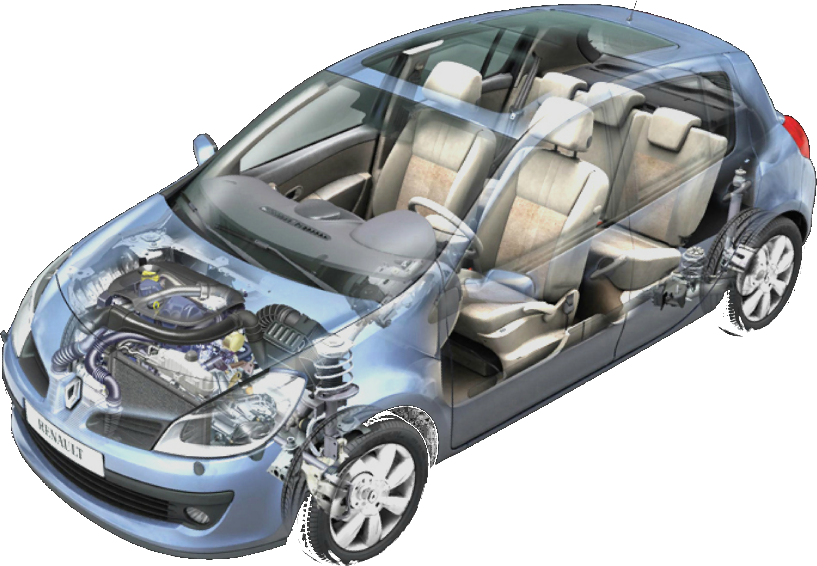
\includegraphics[width=4cm]{png/voiture} &&
%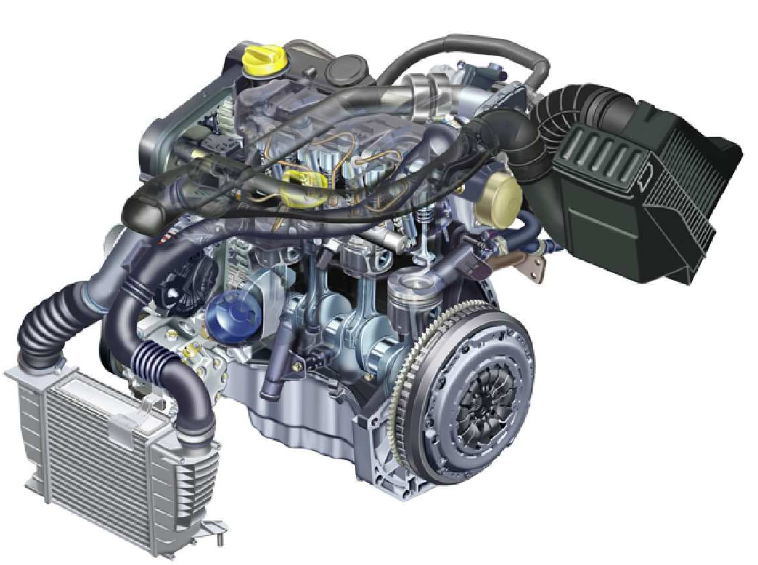
\includegraphics[height=4cm]{png/moteur} && 
%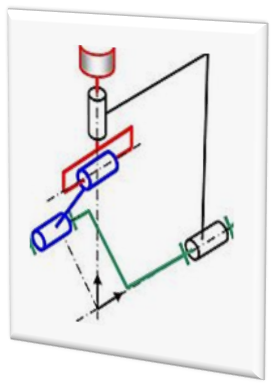
\includegraphics[height=4cm]{png/ex_schema}\\
%\textit{Effeuillage d'un Renault Clio \cite{cite1}} &&
%\textit{Moteur 1.5 dCi K9K 105 ch \cite{cite1}} &&
%\textit{Modélisation par schéma cinématique\cite{cite2}}\\
%\end{tabular}
%\end{center}

\vspace{.2cm}

%
%\begin{obj}
%\textbf{Problématique :}
%\begin{itemize}
%\item M
%\end{itemize}
%\end{obj}

La cinématique du solide indéformable fait intervenir des solides en mouvement relatifs les uns avec les autres. Afin de connaître la position d'un point appartenant à un solide ou la position d'un point appartenant à un autre solide, il est nécessaire de réaliser le paramétrage du système, à partir du schéma cinématique.


\begin{savoir}
\textbf{Savoirs :}
\begin{itemize}
\item Mod - C11.1 Déplacement des points d’un solide : repère lié à un solide, paramètres géométriques linéaires et angulaires définissant la position d'un solide par rapport à un autre, déplacements et petits déplacements d'un solide, torseur des petits déplacements.
\begin{itemize}
\item Mod-C11-S1 : Associer un repère à un solide.
\item Mod-C11-S2 : Identifier les degrés de liberté d’un solide en mouvement par rapport à un repère.
\item Mod-C11-S3 : Réaliser le paramétrage d’un mécanisme simple.
\end{itemize}
\end{itemize}
\end{savoir}

\setlength{\parskip}{0ex plus 0.2ex minus 0ex}
 \renewcommand{\contentsname}{}
 \renewcommand{\baselinestretch}{1}



\textit{Ce document est en évolution permanente. Merci de signaler toutes erreurs ou coquilles.}
\tableofcontents

 \renewcommand{\baselinestretch}{1.2}
\setlength{\parskip}{2ex plus 0.5ex minus 0.2ex}



\section{Paramètres géométriques constants}

\begin{defi}
\textbf{Solide indéformable}

On considère deux points $A$ et $B$ d'un solide indéformable noté $S$. On note $t$ le temps.

$$
\forall A,B \in S, \forall t\in \mathbb{R}, \vect{AB(t)}^2 = \text{constante}
$$

\end{defi}



\begin{defi}
\textbf{Repère orthonormé direct associé à une pièce (ou à une classe d'équivalence cinématique)}

A chacun des solides $(S_i)$ qui constitue un mécanisme on associera une origine $O_i$ ainsi qu'une base orthonormée directe $\left(\vect{x_i};\vect{y_i};\vect{z_i}\right)$. Le point d'origine ainsi que la base forme un repère orthonormé direct nommé $\mathcal{R}_i=\left(O_i;\vect{x_i};\vect{y_i};\vect{z_i}\right)$. 

\end{defi}

\begin{methode}
\textbf{Choix d'un repère lié à une pièce (ou à une classe d'équivalence cinématique)}

On note $\mathcal{R}_i$ le repère associé à la pièce $i$.

\begin{itemize}
\item L'origine du repère sera choisi au centre d'une liaison ou en un point particulier de la classe d'équivalence cinématique. 
\item Le premier axe du repère est, en général, l'axe primaire de la base locale ou la normale de la liaison.
\item Le deuxième axe est perpendiculaire au premier et orienté suivant une direction particulière du sous-ensemble cinématique ou par une direction privilégiée de la liaison (s'il en existe une).
\item Le troisième axe est tel que la base soit orthonormée directe. 
\end{itemize}

Pour choisir un repère lié à une pièce, on choisit un repère dont au moins un vecteur est dans la direction d'un axe d'une des liaisons.
On choisir 
\end{methode}


\begin{defi}
\textbf{Paramétrage géométrique constant}

Soit un solide indéformable auquel on associe un repère $\mathcal{R}$.

Le paramétrage géométrique de ce solide correspond au positionnement des points de ce solide dans le repère $\mathcal{R}$. 
\end{defi}

\begin{exemple}
\textit{Micro compresseur}
\begin{center}
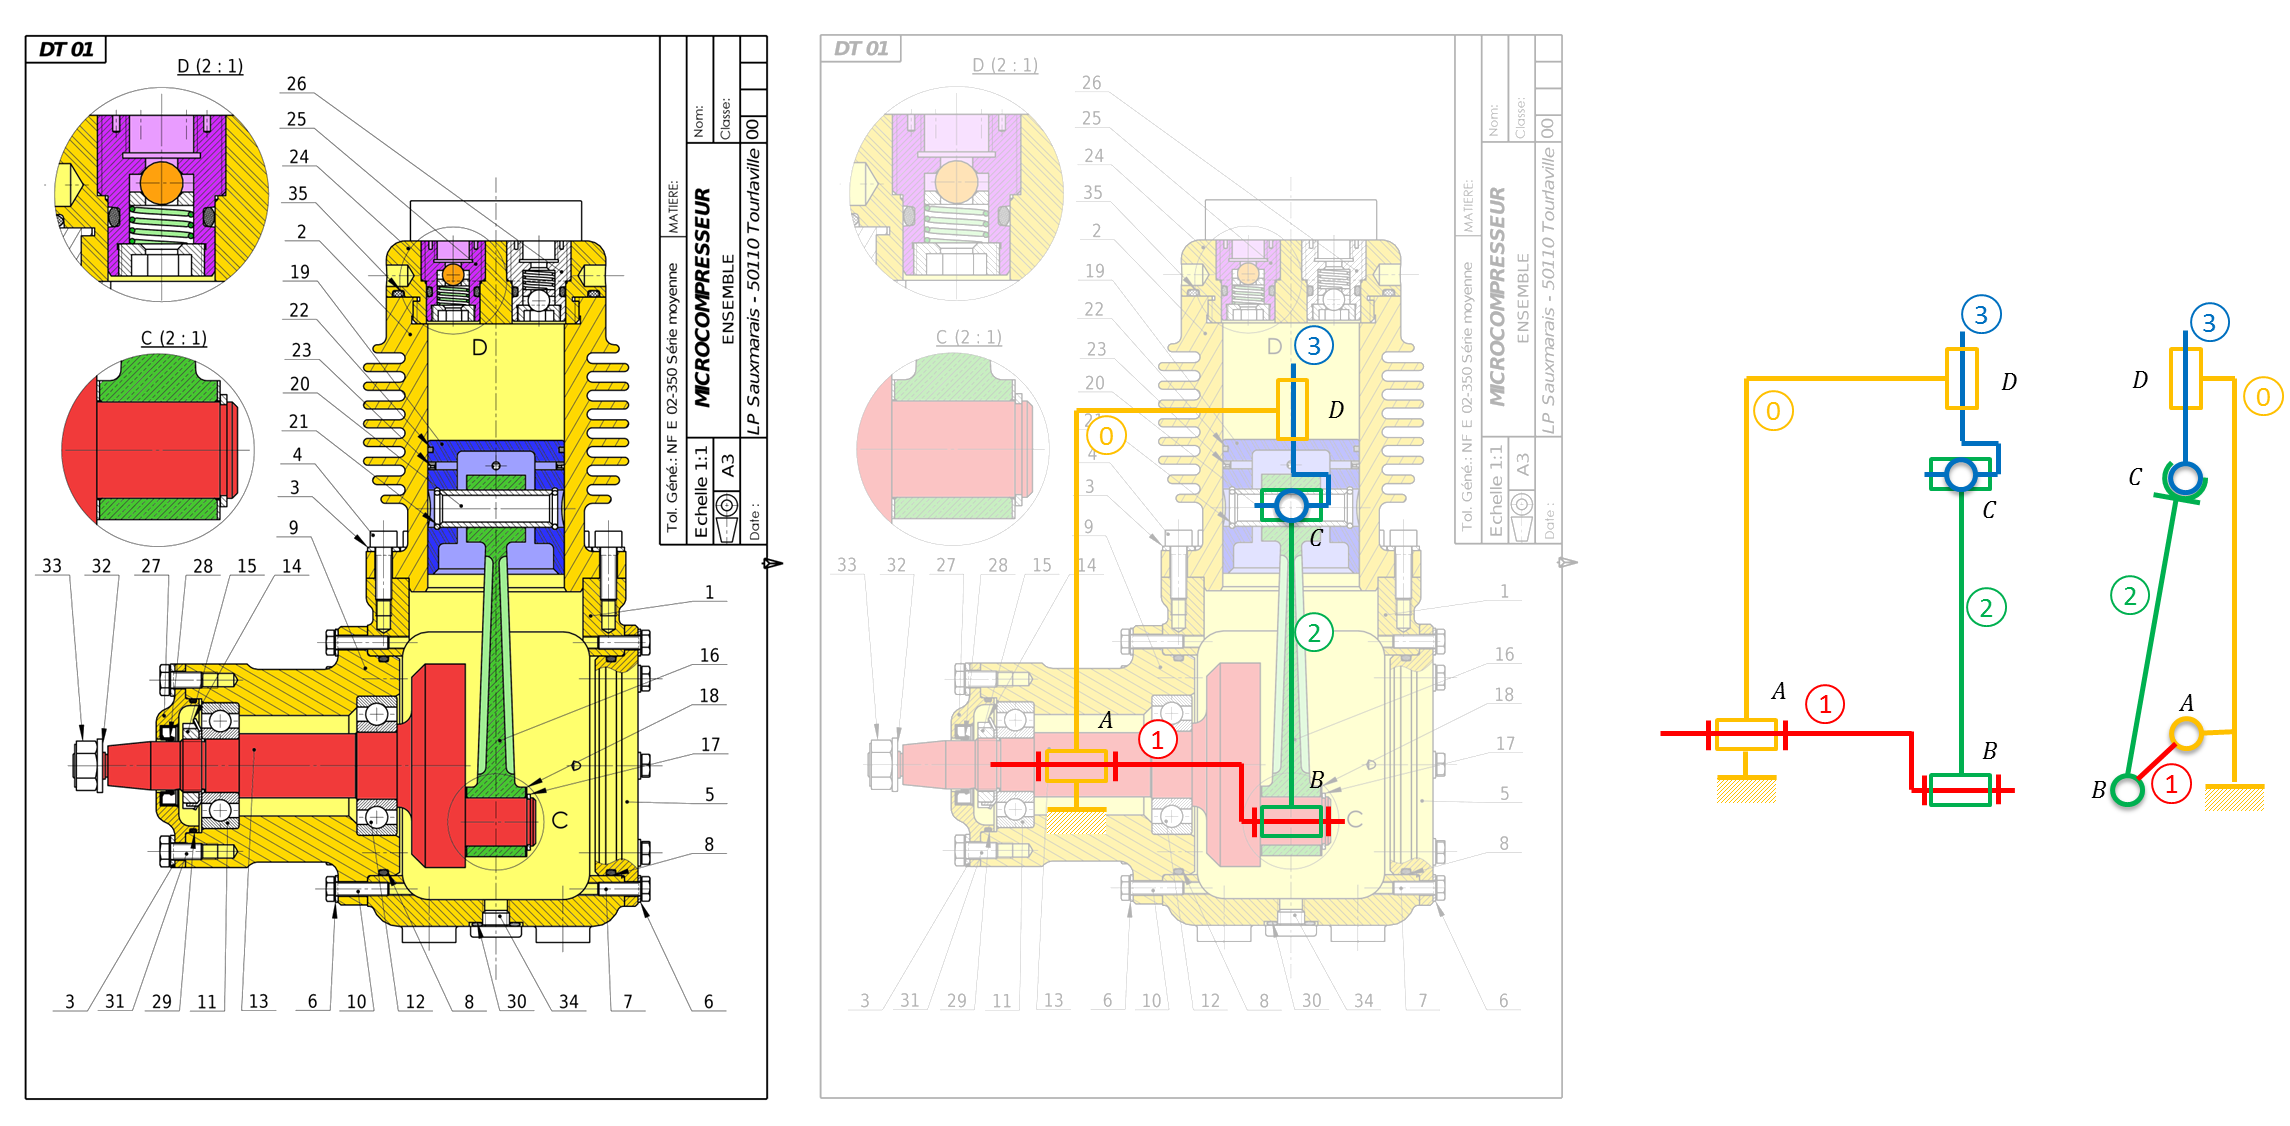
\includegraphics[width=.95\textwidth]{png/modelisme}
\end{center}
\begin{minipage}[c]{.4\linewidth}
On peut donc au bâti 1 le repère orthonormé direct $\mathcal{R}_0=\left(A,\vect{x_0},\vect{y_0},\vect{z_0}\right)$. Le paramétrage du point $D$ est donné par le vecteur $\vect{AD}=x_D\vect{x_0} + y_D\vect{y_0}$.
\end{minipage} \hfill
\begin{minipage}[c]{.55\linewidth}
\begin{center}
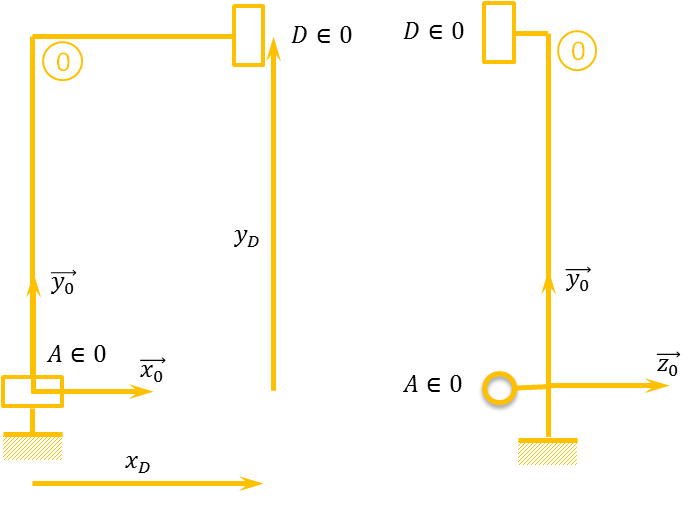
\includegraphics[width=.95\textwidth]{png/solide_0}
\end{center}
\end{minipage}
\end{exemple}

\begin{rem}
Les valeurs des paramètres constants sont constants est positifs. On pourra utiliser des lettres de l'alphabet latin pour désigner les paramètres. 
\end{rem}

\section{Paramètres géométriques variables}
\subsection{Présentation}
\begin{defi}
Dans les systèmes mécaniques, les différentes classes d'équivalence cinématique sont reliées par des liaisons. Ces liaisons possèdent des degrés de liberté. Le but du paramétrage est de définir un paramètre géométrique pour chacun des degrés de liberté de chacune des liaisons. 
\end{defi}

\subsection{Paramétrage d'une translation}

\begin{methode}
Pour paramétrer un degré de liberté en translation il faut définir un paramètre linéaire orienté exprimé en mètres. Le paramètre est une variable qui, en cinématique, dépendra du temps (noté $t$).
\end{methode}

\begin{exemple}
\textit{Paramétrage d'une liaison glissière}

\begin{minipage}[c]{.75\linewidth}
La liaison glissière possède un degré de liberté, à savoir une translation. Ici la position du solide 2 par rapport au solide 1 est définie par le paramètre $\lambda(t)$. On a : 
$$
\vect{O_1 O_2} = \lambda(t) \vect{x_1}
$$
\end{minipage} \hfill
\begin{minipage}[c]{.2\linewidth}
\begin{center}
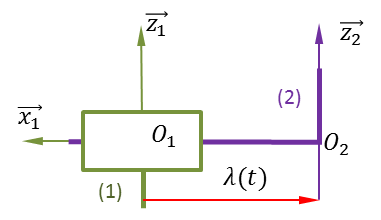
\includegraphics[width=.95\textwidth]{png/glissiere_p}
\end{center}
\end{minipage}
\end{exemple}

\begin{rem}
\begin{itemize}
\item Les paramètres linéaires sont généralement notés par des lettres grecques ($\lambda$, $\mu$ ...).
\item Lorsqu'on paramètre la translation entre un repère $\mathcal{R}_0$ et un repère $\mathcal{R}_1$, les bases sont les mêmes. 
\item Un paramètre linéaire variable changeant de signe au cours du temps sera choisi avec son origine située sur le solide fixe (type bâti) s'il y en a un.
\end{itemize}
\end{rem}



\subsection{Paramétrage d'une rotation}

\begin{methode}
Pour paramétrer un degré de liberté en rotation il faut définir un paramètre angulaire orienté exprimé en radians. Le paramètre est une variable qui, en cinématique, dépendra du temps (noté $t$).

Pour un paramètre angulaire on donnera toujours une figure plane (géométrale) permettant d'illustrer la rotation entre les deux repères.
\end{methode}



\begin{exemple}
\textit{Paramétrage d'une liaison pivot}

\begin{minipage}[c]{.45\linewidth}
La liaison pivot entre les pièces 0 et 1 possède 1 degré de liberté, à savoir une rotation. Ici la position du solide 2 par rapport au solide 1 est définie par le paramètre $\alpha(t)$.
\end{minipage} \hfill
\begin{minipage}[c]{.5\linewidth}
\begin{center}
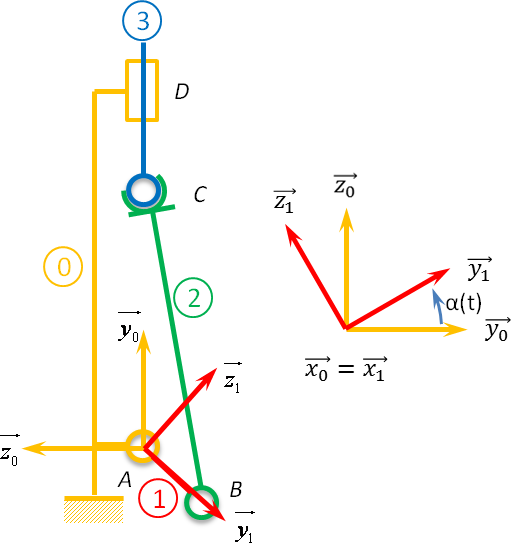
\includegraphics[width=.95\textwidth]{png/pivot_p}
\end{center}
\end{minipage}
\end{exemple}

\subsection{Utilisation des angles d'Euler}

\begin{methode}
Lorsqu'il existe plusieurs rotations entre 2 solides, il faut faire un choix pour paramétrer les 3 rotations (c'est à dire, pour chacune des rotations, on se demande autour de quel axe on doit tourner). Pour paramétrer 3 rotations, on utilise classiquement les angles d'Euler. Ainsi pour passer du repère $\mathcal{R}_0$ au repère $\mathcal{R}_1$ on procède ainsi.

\begin{enumerate}
\item La première rotation est appelée précession. Par une rotation d'angle $\psi(t)$ autour de $\vect{Z_0}$ on passe du repère $\left( \vect{X_0};\vect{Y_0};\vect{Z_0}\right)$ au repère $\left( \vect{u};\vect{v};\vect{Z_0}\right)$.
\item La seconde rotation est appelée nutation. Par une rotation d'angle $\theta(t)$ autour de $\vect{u}$ on passe du repère $\left( \vect{u};\vect{v};\vect{Z_0}\right)$ au repère $\left( \vect{u};\vect{w};\vect{Z_1}\right)$.
\item La dernière rotation est appelée rotation propre. Par une rotation d'angle $\varphi(t)$ autour de $\vect{Z_1}$ on passe du repère $\left( \vect{u};\vect{w};\vect{Z_1}\right)$ au repère $\left( \vect{X_1};\vect{Y_1};\vect{Z_1}\right)$.
\end{enumerate}

\begin{center}
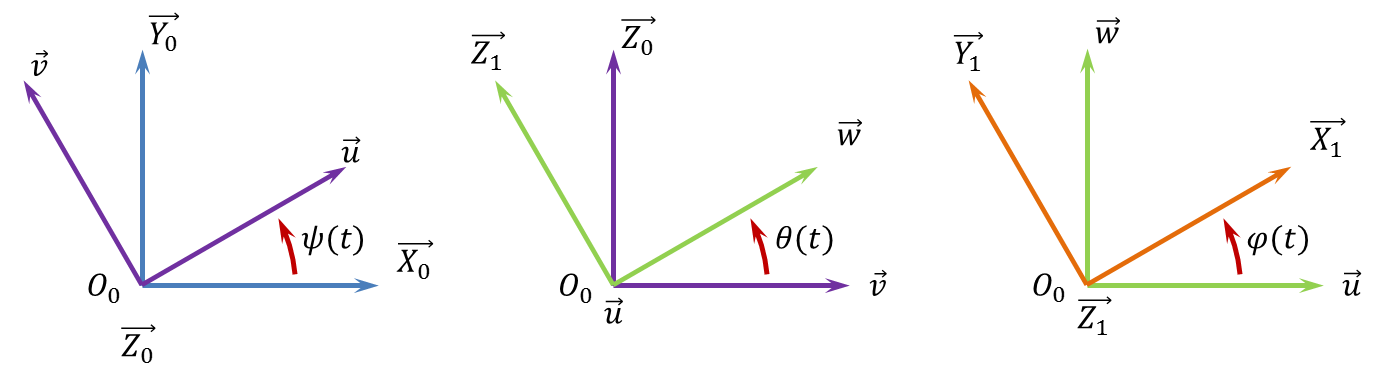
\includegraphics[width=.9\textwidth]{png/param_euler}
\end{center}
\end{methode}

\subsection{Paramétrage des liaisons cinématique}

\subsubsection{Paramétrage de la liaison glissière}
\begin{minipage}[c]{.3\linewidth}
\begin{center}
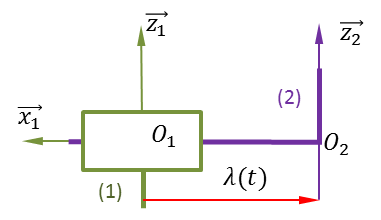
\includegraphics[height=3cm]{png/glissiere_p}
\end{center}
\end{minipage} \hfill
\begin{minipage}[c]{.65\linewidth}
$$
\vect{O_1 O_2} = \lambda(t) \vect{x_1}
$$
\end{minipage}
\subsubsection{Paramétrage de la liaison pivot}
\begin{minipage}[c]{.3\linewidth}
\begin{center}
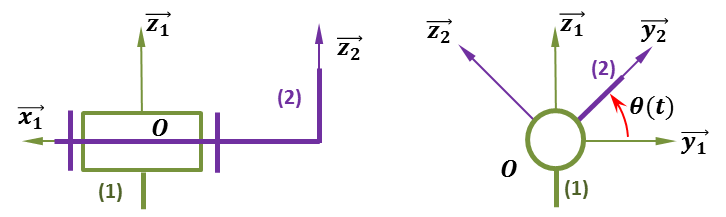
\includegraphics[height=3cm]{png/pivot_p2}
\end{center}
\end{minipage} \hfill
\begin{minipage}[c]{.65\linewidth}

\end{minipage}
\subsubsection{Paramétrage de la liaison glissière hélicoïdale}
\begin{minipage}[c]{.3\linewidth}
\begin{center}
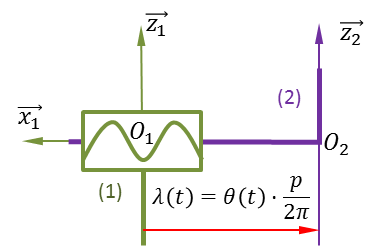
\includegraphics[height=3cm]{png/helico_p}
\end{center}
\end{minipage} \hfill
\begin{minipage}[c]{.65\linewidth}
$$
\vect{O_1 O_2} = \lambda(t) \vect{x_1}
$$
\end{minipage}

\subsubsection{Paramétrage de la liaison pivot glissant}
\begin{minipage}[c]{.3\linewidth}
\begin{center}
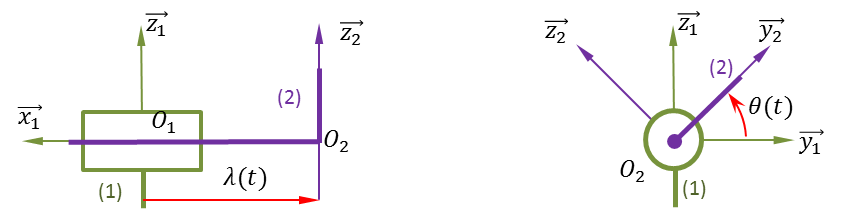
\includegraphics[height=3cm]{png/pivotg_p}
\end{center}
\end{minipage} \hfill
\begin{minipage}[c]{.65\linewidth}

\end{minipage}

\subsubsection{Paramétrage de la liaison rotule à doigt}
\begin{minipage}[c]{.3\linewidth}
\begin{center}
%\includegraphics[height=3cm]{png/}
\end{center}
\end{minipage} \hfill
\begin{minipage}[c]{.65\linewidth}

\end{minipage}

\subsubsection{Paramétrage de la liaison appui plan}
\begin{minipage}[c]{.3\linewidth}
\begin{center}
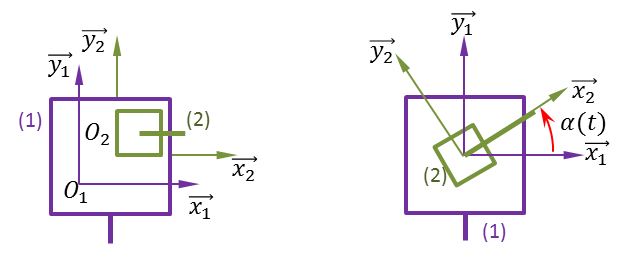
\includegraphics[height=3cm]{png/plan_p}
\end{center}
\end{minipage} \hfill
\begin{minipage}[c]{.65\linewidth}
$$
\vect{O_1 O_2} = \lambda(t) \vect{x_1} + \mu(t) \vect{x_1}
$$
\end{minipage}

\subsubsection{Paramétrage de la liaison sphérique (rotule)}
\begin{minipage}[c]{.3\linewidth}
\begin{center}
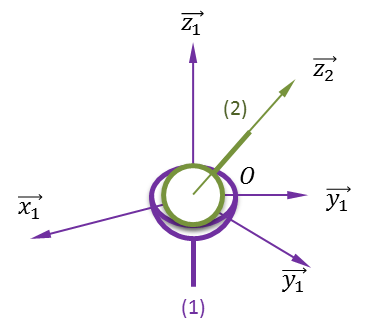
\includegraphics[height=3cm]{png/rotule_3d}
\end{center}
\end{minipage} \hfill
\begin{minipage}[c]{.65\linewidth}
$$
\vect{O_1 O_2} = \lambda(t) \vect{x_1}
$$
\end{minipage}

\subsubsection{Paramétrage de la liaison sphère -- cylindre (linéaire annulaire)}
\begin{minipage}[c]{.3\linewidth}
\begin{center}
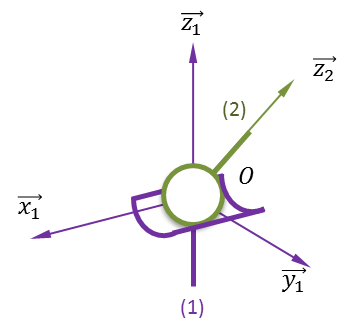
\includegraphics[height=3cm]{png/annulaire_3d}
\end{center}
\end{minipage} \hfill
\begin{minipage}[c]{.65\linewidth}

\end{minipage}

\subsubsection{Paramétrage de la liaison cylindre -- plan}
\begin{minipage}[c]{.3\linewidth}
\begin{center}
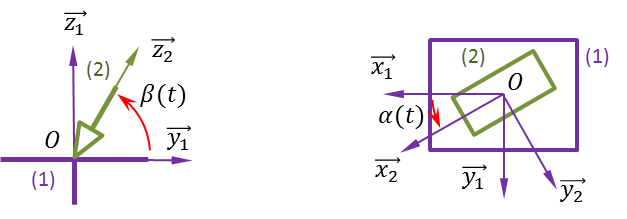
\includegraphics[height=3cm]{png/rectiligne_p}
\end{center}
\end{minipage} \hfill
\begin{minipage}[c]{.65\linewidth}
$$
\vect{O_1 O_2} = \lambda(t) \vect{x_1} + \mu(t) \vect{x_1}
$$
\end{minipage}

\subsubsection{Paramétrage de la liaison sphère -- plan (ponctuelle)}
\begin{minipage}[c]{.3\linewidth}
\begin{center}
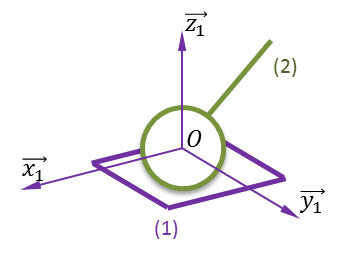
\includegraphics[height=3cm]{png/ponctuelle_3d}
\end{center}
\end{minipage} \hfill
\begin{minipage}[c]{.65\linewidth}
$$
\vect{O_1 O_2} = \lambda(t) \vect{x_1} + \mu(t) \vect{x_1}
$$
\end{minipage}



\begin{thebibliography}{2}
\bibitem[1]{JPP} Jean-Pierre Pupier -- Paramétrage -- PTSI -- Lycée Rouvière Toulon.
\end{thebibliography}
\end{document}

